\chapter{Biologia estrutural das proteínas}\label{ch:b3:structural-biology}

Max Perutz começou a trabalhar na estrutura da hemoglobina em 1937 e a
publicou em 1960: vinte e dois anos para ver, a uma \omterm{def:b3:structural-biology:methods}{resolução} de meio
nanômetro, como quatro cadeias de cento e cinquenta aminoácidos se
dobram em torno de quatro hemes. Uma molécula de hemoglobina se dobra
sozinha em alguns milissegundos. Entre esses dois fatos está o assunto
deste capítulo: o que é a forma de uma proteína, por que uma cadeia de
aminoácidos tem uma forma e não outra, como ela encontra essa forma tão
depressa entre um número astronômico de alternativas, o que dá errado
quando não a encontra, como as formas são vistas --- por raios X, por
ressonância magnética, por elétrons e, hoje, por computação --- e como
uma proteína se move entre formas para fazer seu trabalho, com a troca
da hemoglobina entre uma forma tensa e uma relaxada como modelo de toda
proteína alostérica desde então.

\section{O que é a estrutura de uma proteína}

\begin{definition}[Níveis de estrutura]\label{def:b3:structural-biology:levels}
\index{estrutura secundária}\index{hélice alfa}\index{folha beta}\index{estrutura terciária}\index{domínio}\index{enovelamento}
A \emph{estrutura primária} é a sequência de resíduos. A
\emph{estrutura secundária} é a conformação regular local do esqueleto,
estabilizada por pontes de hidrogênio entre as carbonilas e as amidas
do esqueleto: a \emph{$\alpha$-hélice}, uma espiral dextrógira de $3.6$
resíduos por volta, que sobe \qty{0.15}{nm} por resíduo
(\qty{0.54}{nm} por volta), cada carbonila ligada à amida quatro
resíduos adiante; e a \emph{folha~$\beta$}, em que fitas estendidas se
dispõem lado a lado, paralelas ou antiparalelas, ligadas às vizinhas,
com as cadeias laterais alternando acima e abaixo da folha. A
\emph{estrutura terciária} é o enovelamento de uma cadeia inteira em
três dimensões; uma unidade compacta que se dobra de modo independente,
de \numrange{50}{250} resíduos dentro dela, é um \emph{domínio}, e o
arranjo dos elementos secundários de um domínio é seu
\emph{enovelamento}. A \emph{estrutura quaternária} é a montagem de
várias cadeias: o $\alpha_{2}\beta_{2}$ da hemoglobina. Cerca de
\num{1300} enovelamentos dão conta de todos os domínios conhecidos, e
algumas dezenas deles --- o enovelamento de Rossmann, o barril TIM, o
enovelamento de imunoglobulina --- de uma grande fração de todas as
proteínas: a natureza reaproveita enovelamentos e varia suas
sequências.
\end{definition}

\begin{omfigure}
\begin{tikzpicture}
\begin{axis}[
  width=6.4cm, height=6.4cm,
  xmin=-180, xmax=180, ymin=-180, ymax=180,
  xlabel={$\phi$ (graus)}, ylabel={$\psi$ (graus)},
  xlabel style={font=\small}, ylabel style={font=\small},
  tick label style={font=\scriptsize}, xtick={-180,-90,0,90,180}, ytick={-180,-90,0,90,180},
  axis lines=box, grid=major, grid style={gray!25},
  clip=false,
]
% beta region
\fill[omDef!30] (axis cs:-180,90) rectangle (axis cs:-45,180);
\fill[omDef!30] (axis cs:-180,-180) rectangle (axis cs:-45,-150);
\node[font=\scriptsize, omDef!60!black] at (axis cs:-112,165) {fitas $\beta$};
% alpha R region
\fill[omThm!30] (axis cs:-160,-70) rectangle (axis cs:-45,0);
\node[font=\scriptsize, omThm!70!black] at (axis cs:-105,-58) {$\alpha$ dextrógira};
% alpha L region
\fill[omMeth!30] (axis cs:45,0) rectangle (axis cs:100,80);
\node[font=\scriptsize, omMeth!60!black, align=center] at (axis cs:72,40) {levó-\\gira};
\addplot[only marks, mark=*, mark size=1pt, black] coordinates {(-57,-47)};
\node[font=\scriptsize, anchor=south west] at (axis cs:-52,-44) {$\alpha$: $(-57,-47)$};
\addplot[only marks, mark=*, mark size=1pt, black] coordinates {(-139,135)};
\node[font=\scriptsize, anchor=west] at (axis cs:-134,135) {$\beta$ antiparalela};
\end{axis}
\node[align=left, font=\scriptsize, anchor=west] at (7.0,3.0) {Os dois ângulos de torção do esqueleto de cada\\resíduo, $\phi$ (em torno de N--C$_\alpha$) e $\psi$ (em torno\\de C$_\alpha$--C), são restringidos por choques estéricos\\às regiões coloridas. Uma hélice põe cada resíduo\\num mesmo ponto; uma fita, perto de outro.\\A glicina, sem cadeia lateral, alcança mais longe;\\a prolina, com seu anel, fica presa perto de $\phi = -60$.};
\end{tikzpicture}

{\small O diagrama de Ramachandran. As regiões sombreadas são as
combinações estericamente permitidas dos ângulos $\phi$ e $\psi$ do
esqueleto; a $\alpha$-hélice dextrógira e a fita~$\beta$ correspondem
cada uma a uma região pequena, e a maioria dos resíduos de uma proteína
enovelada cai numa delas.}
\end{omfigure}

\begin{proposition}[O que mantém um enovelamento]\label{prop:b3:structural-biology:forces}
\index{efeito hidrofóbico}\index{estabilidade marginal}
Uma proteína enovelada é estabilizada pelo \emph{\omterm{prop:b3:structural-biology:forces}{efeito hidrofóbico}}
--- enterrar cadeias laterais apolares num cerne longe da água, o que
libera as moléculas de água que de outro modo ficariam ordenadas em
torno delas ---, pelas pontes de hidrogênio da \omterm{def:b3:structural-biology:levels}{estrutura secundária} e
de grupos polares enterrados, pelo empacotamento de van der Waals de um
cerne tão denso quanto um cristal, por pontes salinas ocasionais e, nas
proteínas secretadas, por pontes dissulfeto. O \omterm{prop:b3:structural-biology:forces}{efeito hidrofóbico}
fornece a maior parte do impulso; as pontes de hidrogênio em geral se
pagam a si mesmas (um esqueleto ligado à água no estado desenovelado
está ligado a si mesmo no enovelado) e, em vez disso, ditam
\emph{qual} \omterm{def:b3:structural-biology:levels}{enovelamento}. A energia livre líquida do \omterm{def:b3:structural-biology:levels}{enovelamento} é
pequena, $\Delta G \approx -20$ a \qty{-60}{kJ/mol} --- a força de um
punhado de pontes de hidrogênio numa molécula que tem centenas ---
porque a perda de entropia conformacional no \omterm{def:b3:structural-biology:levels}{enovelamento} quase anula o
ganho em entalpia. As proteínas são \emph{marginalmente estáveis}: uns
poucos graus, uma mudança de pH ou uma única mutação no cerne podem
desenovelá-las, e essa marginalidade é o que lhes permite mover-se.
\end{proposition}

\begin{proof}[Evidência]
Anfinsen (1961) desenovelou a ribonuclease~A com ureia e um agente
redutor, rompendo suas quatro pontes dissulfeto e destruindo sua
atividade; ao retirar os dois, a enzima se reenovelou, reformou as
quatro pontes corretas entre os $105$ pareamentos possíveis e
recuperou toda a atividade. Nenhum molde, nenhuma enzima, nenhuma
informação além da sequência estava presente: a estrutura nativa é o
estado termodinamicamente mais estável acessível à cadeia, e a
sequência a codifica. Reoxidar as pontes dissulfeto com a cadeia ainda
em ureia deu uma mistura embaralhada com \qty{1}{\%} de atividade, que
então se desembaralhou até a forma nativa quando lhe permitiram
enovelar-se: a cadeia encontra o mínimo por si só.
\end{proof}

\section{Como uma cadeia encontra seu enovelamento}

\begin{theorem}[O paradoxo de Levinthal]\label{thm:b3:structural-biology:levinthal}
\index{paradoxo de Levinthal}\index{funil de enovelamento}
Se cada um dos $n$ resíduos de uma proteína pudesse adotar $k$
conformações de esqueleto de modo independente, a cadeia teria $k^{n}$
conformações. Com $k = 3$ e $n = 100$ isso dá $3^{100} \approx
5\times 10^{47}$; amostrá-las a uma por picossegundo ($10^{12}$ por
segundo) levaria $5\times 10^{35}$ segundos, cerca de $10^{28}$ anos.
Proteínas desse tamanho se enovelam em milissegundos a segundos. Logo,
o \omterm{def:b3:structural-biology:levels}{enovelamento} não é uma busca ao acaso entre conformações: a
superfície de energia é um \emph{funil}, no qual quase toda conformação
parcial é enviesada rumo ao estado nativo, e a cadeia desce por
movimentos locais que são, em média, cada um ladeira abaixo.
\end{theorem}
\begin{proof}
A contagem é o princípio multiplicativo; o tempo é a contagem dividida
pela taxa de amostragem, $5\times 10^{47}/10^{12} = 5\times
10^{35}$ s,
e um ano tem $3\times 10^{7}$ s. A conclusão é a contrapositiva: uma
busca ao acaso desse tamanho é impossível no tempo observado, logo a
busca não é ao acaso. O que a torna não aleatória é que uma interação
formada numa parte da cadeia persiste enquanto outras se formam (o
colapso hidrofóbico e a formação de hélices acontecem em microssegundos
e reduzem o espaço a percorrer) e que as estruturas parcialmente
corretas têm, em média, energia mais baixa que as erradas, de modo que
a descida é guiada --- um funil, e não um campo de golfe com um único
buraco.
\end{proof}

\begin{omfigure}
\begin{tikzpicture}[every node/.style={font=\scriptsize}, >=stealth]
  % funnel outline
  \draw[very thick, omDef] (-4,3) .. controls (-3.2,1.5) and (-1.2,0.2) .. (-0.35,-1.2) -- (-0.35,-1.6);
  \draw[very thick, omDef] (4,3) .. controls (3.2,1.5) and (1.2,0.2) .. (0.35,-1.2) -- (0.35,-1.6);
  \draw[very thick, omDef] (-0.35,-1.6) -- (0.35,-1.6);
  % rugged inner lines
  \draw[omDef!60, thick] (-3.3,2.6) .. controls (-2.9,2.2) and (-2.6,2.6) .. (-2.2,2.0) .. controls (-1.9,1.5) and (-1.7,1.9) .. (-1.4,1.2) .. controls (-1.1,0.7) and (-0.9,0.9) .. (-0.6,0.2);
  \draw[omDef!60, thick] (3.3,2.6) .. controls (2.9,2.1) and (2.5,2.5) .. (2.1,1.8) .. controls (1.8,1.3) and (1.5,1.6) .. (1.2,1.0) .. controls (1.0,0.6) and (0.8,0.8) .. (0.6,0.2);
  % axes
  \draw[->] (-5.9,-1.8) -- (-5.9,3.2) node[above, align=center] {energia\\livre};
  \draw[<->] (-3.9,3.85) -- (3.9,3.85) node[midway, above] {entropia conformacional (amplitude do conjunto)};
  % labels
  \node[above] at (0,3.05) {cadeia desenovelada: muitas conformações, alta energia};
  \node[right, align=left] at (3.3,1.4) {armadilhas locais: intermediários\\parcialmente mal enovelados};
  \node[left, align=right] at (-3.3,1.4) {colapso rápido e\\estrutura secundária};
  \node[below] at (0,-1.7) {estado nativo: uma conformação, energia mínima};
  \draw[->, thick, omThm] (-2.8,2.4) .. controls (-2.0,1.2) and (-0.8,0.5) .. (-0.15,-1.3);
  \node[omThm, left] at (-1.5,-0.5) {uma trajetória de enovelamento};
\end{tikzpicture}

{\small O \omterm{thm:b3:structural-biology:levinthal}{funil de enovelamento}. A energia livre cai e o número de
conformações disponíveis encolhe à medida que a cadeia se aproxima do
estado nativo; as paredes são acidentadas, de modo que uma cadeia pode
ficar presa num intermediário parcialmente mal enovelado, mas a
inclinação geral a leva até o fundo em milissegundos.}
\end{omfigure}

\begin{definition}[Chaperonas]\label{def:b3:structural-biology:chaperones}
\index{chaperona}\index{Hsp70}\index{chaperonina}\index{GroEL}
Uma \emph{chaperona molecular} é uma proteína que auxilia o
\omterm{def:b3:structural-biology:levels}{enovelamento} de outras sem se tornar parte delas nem fornecer
informação sobre o \omterm{def:b3:structural-biology:levels}{enovelamento}: ela impede a agregação que compete com
o \omterm{def:b3:structural-biology:levels}{enovelamento} no citoplasma abarrotado. A \emph{Hsp70} liga segmentos
hidrofóbicos expostos de cadeias nascentes ou desenoveladas e as libera
com a hidrólise de ATP para nova tentativa; a \emph{chaperonina} GroEL
(Hsp60 nas mitocôndrias, TRiC no citosol eucarionte) é um barril duplo
de catorze subunidades cuja cavidade central, tampada pela GroES,
encerra uma única cadeia de até \qty{60}{kDa} em isolamento por cerca
de dez segundos --- uma gaiola de Anfinsen --- e a ejeta enovelada ou
não, para tentar de novo. Cerca de um décimo das proteínas bacterianas
recém-feitas passa pela GroEL, e uma célula cujas chaperonas são
sobrecarregadas --- pelo calor, razão pela qual a maioria delas são
\emph{proteínas de choque térmico} induzidas por uma elevação da
temperatura --- enche-se de agregados.
\end{definition}

\begin{definition}[Amiloide]\label{def:b3:structural-biology:amyloid}
\index{amiloide}\index{cross-beta}\index{príon}\index{doença de mau enovelamento}
O \emph{amiloide} é um agregado ordenado de proteína em que as cadeias
se empilham em fibrilas não ramificadas de \qtyrange{5}{10}{nm} de
largura, com as fitas de cada cadeia correndo perpendicularmente ao
eixo da fibrila e ligadas por pontes de hidrogênio às fitas da cadeia
seguinte --- a estrutura \emph{cross-$\beta$}, a mesma seja qual for a
proteína. Quase qualquer proteína pode formá-lo em condições
desestabilizantes; nas \emph{doenças de mau \omterm{def:b3:structural-biology:levels}{enovelamento}} determinadas
proteínas o fazem no corpo: a amiloide-$\beta$ e a tau na doença de
Alzheimer, a $\alpha$-sinucleína na de Parkinson, a huntingtina, a
transtirretina, o amiloide das ilhotas no diabetes tipo~2. Um
\emph{príon} é um amiloide que se propaga: a forma mal enovelada da
proteína priônica PrP converte a forma normal, por contato, em mais de
si mesma, de modo que a ``infecção'' não carrega ácido nucleico algum,
apenas uma forma --- o mecanismo do scrapie, da encefalopatia
espongiforme bovina e da doença de Creutzfeldt--Jakob, estabelecido por
Prusiner a partir de 1982 contra longa resistência.
\end{definition}

\begin{omfigure}
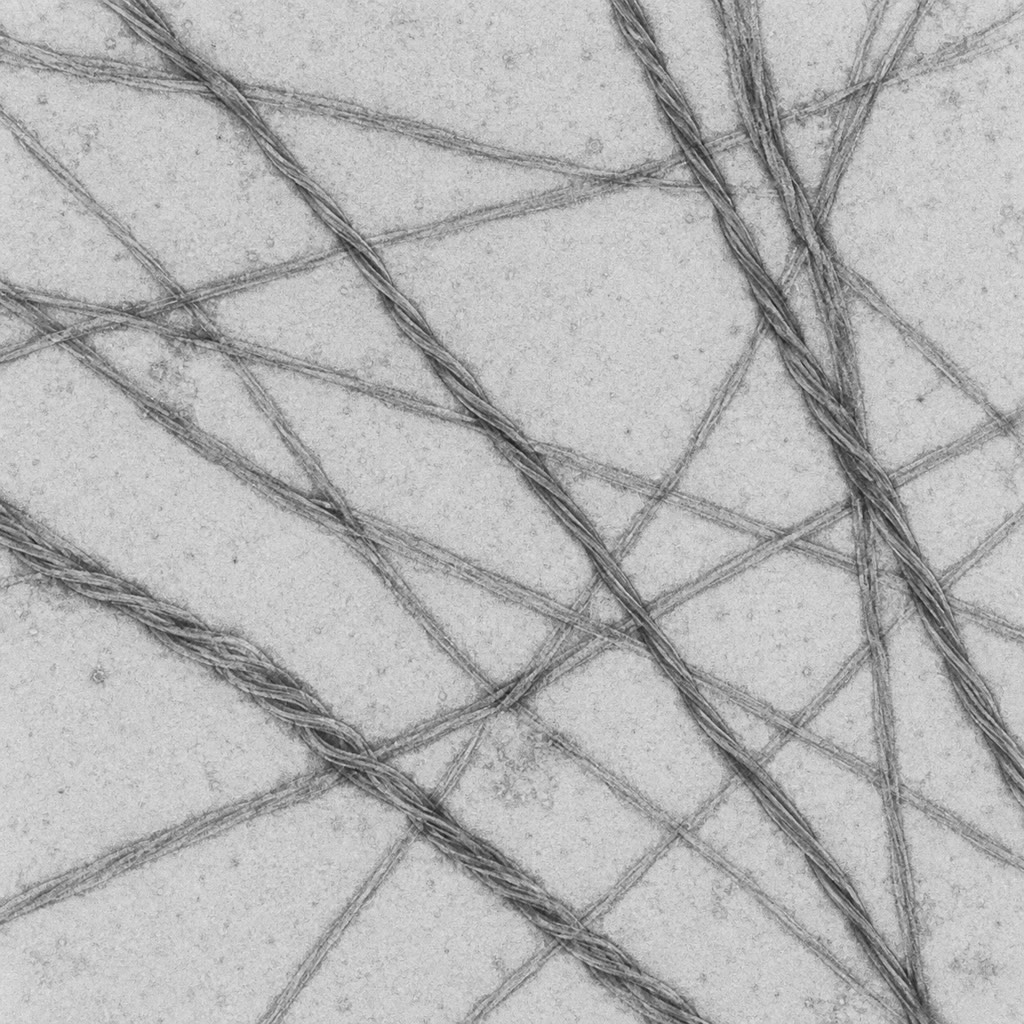
\includegraphics[width=0.36\linewidth]{images/book5/ai/b5-07-amyloid-fibrils.jpg}\hspace{0.04\linewidth}
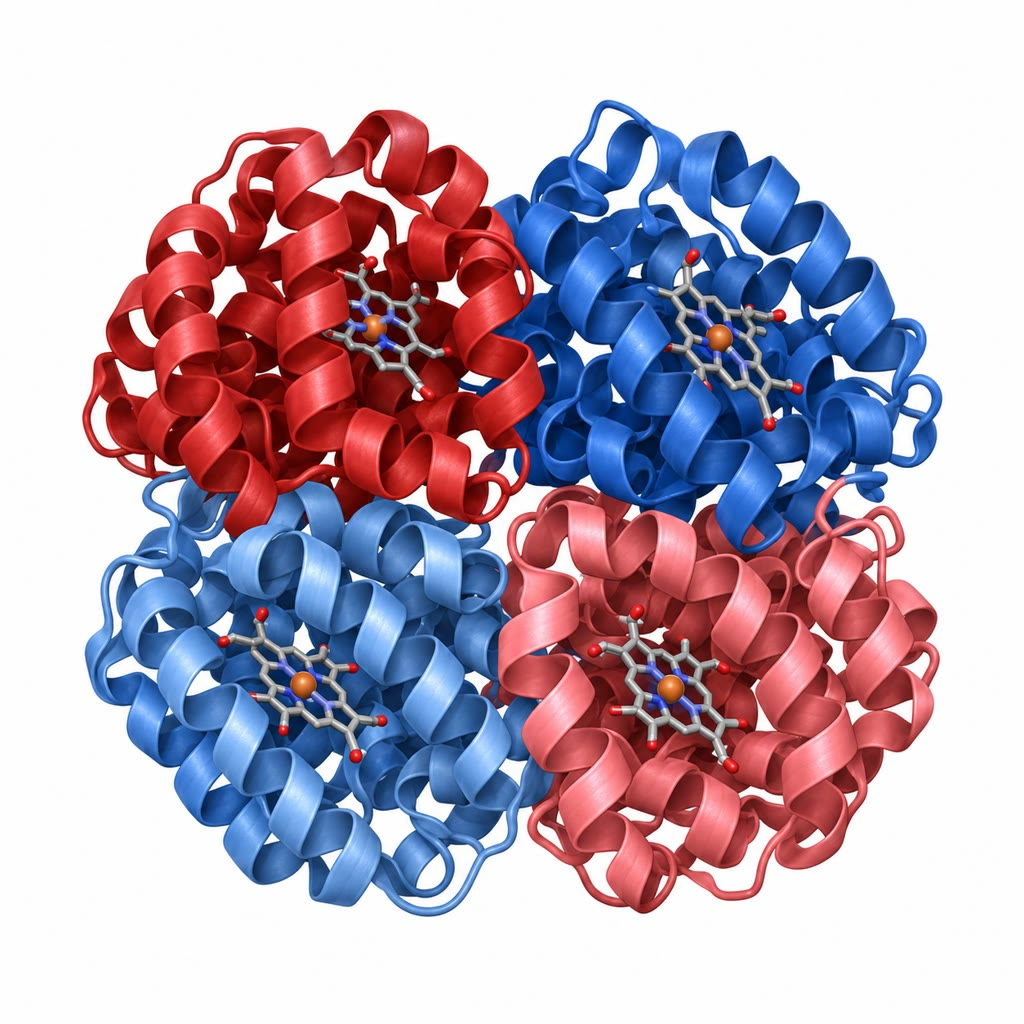
\includegraphics[width=0.36\linewidth]{images/book5/ai/b5-07-haemoglobin-model.jpg}

{\small À esquerda: fibrilas \omterm{def:b3:structural-biology:amyloid}{amiloides} no microscópio eletrônico ---
retas, não ramificadas, às vezes torcidas, e estruturalmente parecidas
seja qual for a proteína de que são feitas. À direita: o tetrâmero da
hemoglobina, duas cadeias $\alpha$ e duas $\beta$, cada uma abrigando
um heme.}
\end{omfigure}

\section{Ver uma proteína}

\begin{definition}[Métodos estruturais]\label{def:b3:structural-biology:methods}
\index{cristalografia de raios X}\index{espectroscopia de RMN}\index{criomicroscopia eletrônica}\index{resolução}
A \emph{cristalografia de raios X} cresce um cristal da proteína,
expõe-no a um feixe de raios X e registra o padrão de difração; as
posições dos pontos dão a rede e suas intensidades, uma vez recuperadas
as fases das ondas, dão a densidade eletrônica da célula unitária, na
qual a cadeia é construída. A \emph{ressonância magnética nuclear}
(RMN) mede, em solução, os acoplamentos entre os núcleos de átomos
próximos no espaço, a partir dos quais se calculam distâncias e daí uma
estrutura; ela funciona para proteínas abaixo de uns \qty{40}{kDa} e
informa sobre seus movimentos. A \emph{criomicroscopia eletrônica}
fotografa de milhares a milhões de moléculas isoladas congeladas num
filme fino de gelo vítreo, cada uma em orientação aleatória, e
reconstrói a densidade tridimensional combinando-as; desde os
detectores diretos de elétrons (2013) ela alcança resolução atômica e
não precisa de cristal, de modo que complexos grandes, proteínas de
membrana e montagens flexíveis que nunca cristalizaram são hoje
resolvidos de rotina. A \emph{resolução} de uma estrutura é o menor
espaçamento em que dois detalhes ficam separados: a \qty{0.35}{nm} o
esqueleto e as cadeias laterais grandes são posicionados, a
\qty{0.2}{nm} cada átomo, a \qty{0.1}{nm} os hidrogênios.
\end{definition}

\begin{proof}[Evidência]
Kendrew (1958) obteve a primeira estrutura de uma proteína, a
mioglobina de cachalote, a \qty{0.6}{nm} --- uma salsicha de
irregularidade inesperada, ``mais complicada e menos simétrica do que
qualquer um previra'' --- e a \qty{0.2}{nm} em 1960, quando as
$\alpha$-hélices que Pauling propusera a partir de modelos em 1951
foram vistas pela primeira vez. Perutz (1960) resolveu a hemoglobina a
\qty{0.55}{nm} usando o método de átomos pesados que idealizara para
obter as fases: átomos de mercúrio presos à proteína mudam as
intensidades de um modo que revela a informação que falta. Comparando
as formas oxigenada e desoxigenada (1970), ele viu as subunidades
girarem umas contra as outras em \qty{15}{\degree} ao ligar o
oxigênio, a primeira transição alostérica observada em escala atômica.
\end{proof}

\begin{omfigure}
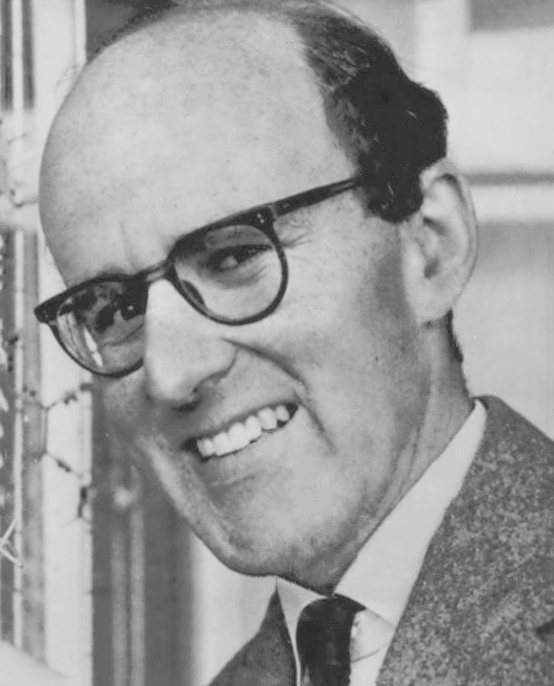
\includegraphics[width=0.30\linewidth]{images/book5/perutz.jpg}\hspace{0.04\linewidth}
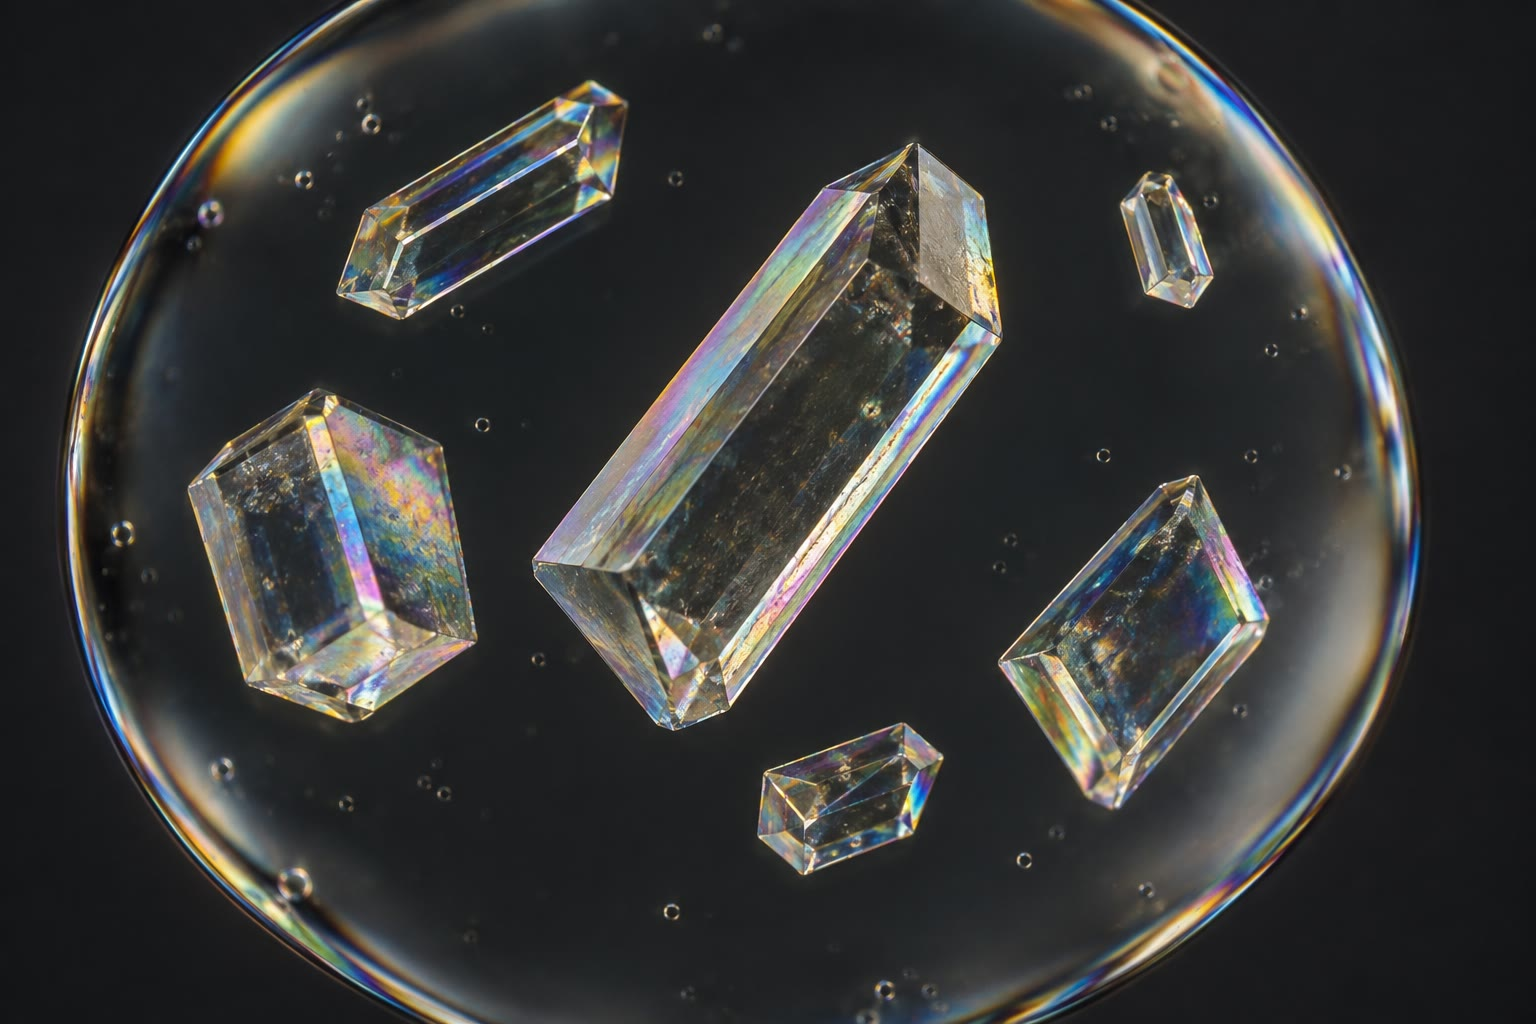
\includegraphics[width=0.30\linewidth]{images/book5/ai/b5-07-protein-crystals.jpg}\hspace{0.04\linewidth}
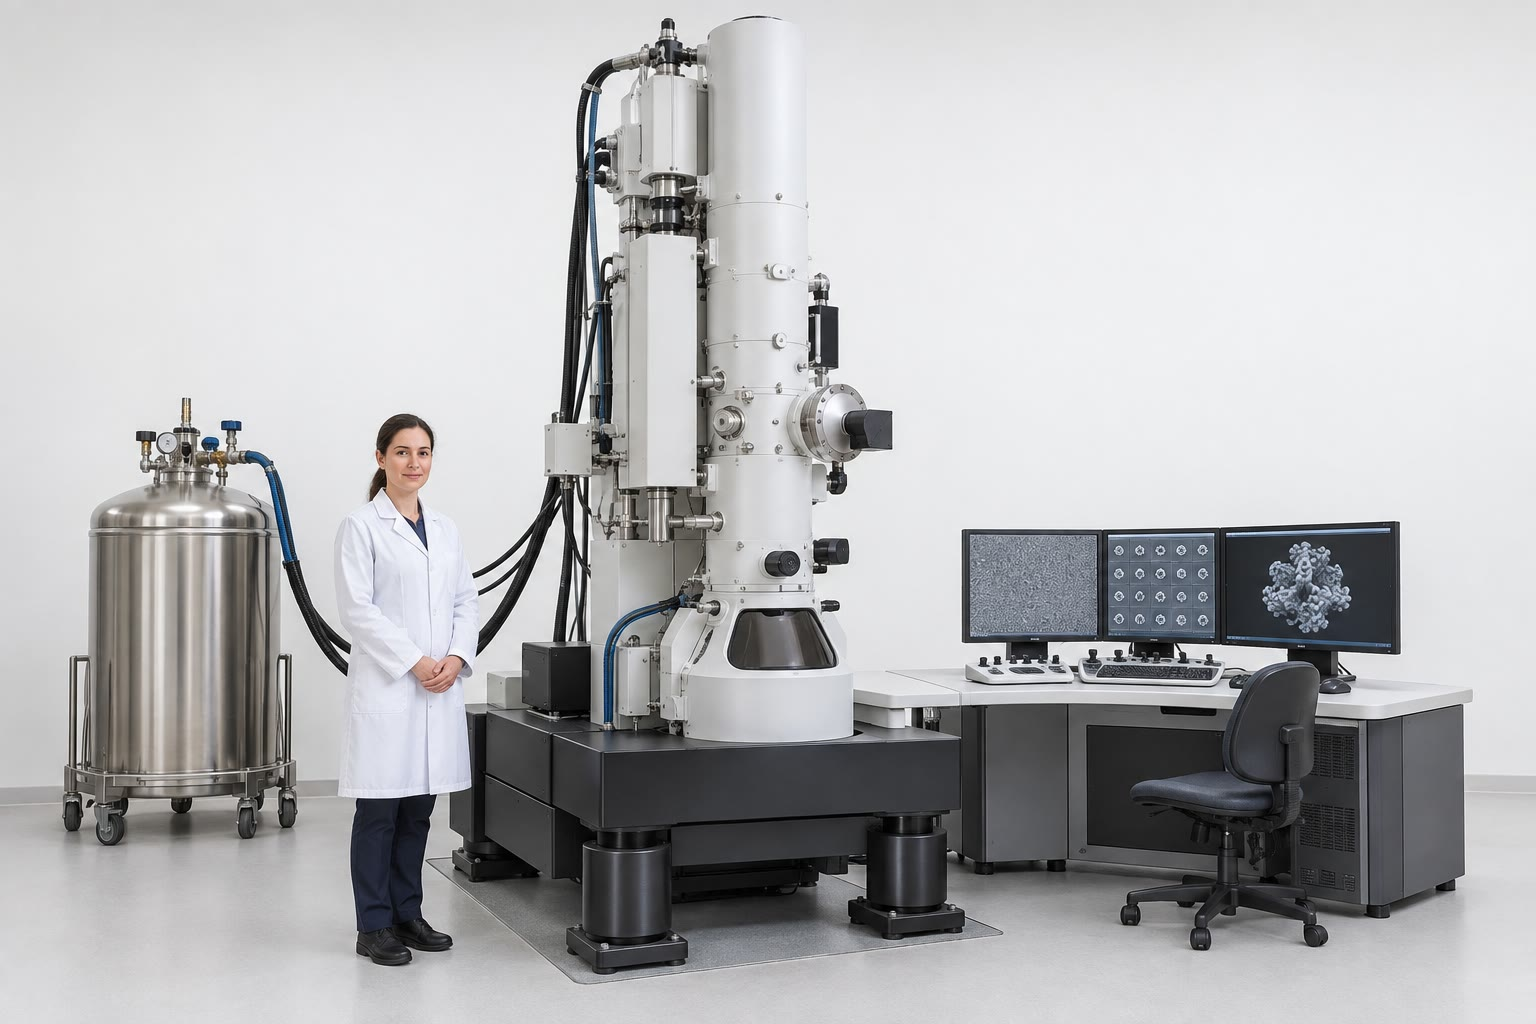
\includegraphics[width=0.30\linewidth]{images/book5/ai/b5-07-cryo-em.jpg}

{\small Max Perutz em 1962, ano de seu prêmio Nobel pela estrutura da
hemoglobina (Associated Press, \omterm{def:b3:structural-biology:levels}{domínio} público). Ao centro: cristais de
proteína numa gota suspensa, o ponto de partida da cristalografia. À
direita: um criomicroscópio eletrônico, o instrumento que tornou os
cristais desnecessários.}
\end{omfigure}

\begin{method}[Resolver uma estrutura por cristalografia]\label{met:b3:structural-biology:crystallography}
\index{lei de Bragg}\index{problema das fases}
(1) Purifique miligramas da proteína e teste centenas de condições
(precipitante, pH, sal) em busca de cristais; (2) congele rapidamente
um cristal e colete imagens de difração num síncrotron enquanto ele
gira no feixe; (3) indexe os pontos para obter a célula unitária e a
simetria; o maior ângulo em que se veem pontos fixa a \omterm{def:b3:structural-biology:methods}{resolução} pela
\omterm{met:b3:structural-biology:crystallography}{lei de Bragg}, $d =
\lambda/(2\sin\theta)$; (4) resolva o \emph{problema
das fases} --- o detector registra intensidades, mas não fases --- com
átomos pesados, com o espalhamento anômalo do selênio na
selenometionina, ou, para uma proteína parecida com outra já conhecida,
por substituição molecular, colocando o modelo conhecido na célula; (5)
calcule a densidade eletrônica, construa a cadeia dentro dela e refine
o modelo contra os dados até que a discordância (fator~$R$) seja
pequena; (6) valide: geometria, discrepâncias de Ramachandran e o
ajuste a dados contra os quais o modelo não foi refinado.
\end{method}

\begin{omfigure}
\begin{tikzpicture}[every node/.style={font=\scriptsize}, >=stealth]
  % crystal
  \draw[thick, fill=omDef!20] (0,0) -- (1.4,0) -- (1.9,0.6) -- (0.5,0.6) -- cycle; \draw[thick, fill=omDef!30] (0,0) -- (0.5,0.6) -- (0.5,1.6) -- (0,1.0) -- cycle; \draw[thick, fill=omDef!25] (0.5,0.6) -- (1.9,0.6) -- (1.9,1.6) -- (0.5,1.6) -- cycle;
  \node[below] at (0.95,-0.1) {cristal: $10^{12}$ moléculas alinhadas};
  % beam
  \draw[->, very thick, omThm] (-2.2,0.9) -- (-0.1,0.9); \node[above] at (-1.2,0.95) {raios X, $\lambda \approx \qty{0.1}{nm}$};
  % diffracted beams
  \foreach \a in {-25,-12,5,18,30} \draw[->, omThm, thick] (1.9,0.9) -- ++(\a:3.2);
  % detector
  \draw[thick] (5.2,-1.2) rectangle (5.6,3.0); \node[right, align=left] at (5.7,2.6) {detector: pontos em\\ângulos $\theta$, com\\intensidades $I$};
  \foreach \y in {-0.6,-0.1,0.6,1.2,1.9,2.4} \fill[black] (5.4,\y) circle (0.06);
  % arrow to density
  \draw[->, very thick] (7.4,0.9) -- (8.6,0.9) node[midway, above, align=center] {fases\\recuperadas};
  \node[right, align=left] at (8.7,1.4) {densidade eletrônica};
  \draw[omDef, thick] (8.8,0.4) .. controls (9.1,1.1) and (9.5,0.2) .. (9.8,0.8) .. controls (10.1,1.3) and (10.4,0.3) .. (10.7,0.9);
  \node[right, align=left] at (8.7,-0.4) {modelo construído nela,\\refinado, validado};
  % Bragg
  \node[anchor=north west, align=left] at (-2.2,-0.7) {Bragg: $2d\sin\theta = \lambda$ ---\\o maior $\theta$ observado fixa a resolução $d$};
\end{tikzpicture}

{\small Do cristal ao modelo. A rede regular espalha os raios X em
pontos discretos; o ponto de maior ângulo fixa a \omterm{def:b3:structural-biology:methods}{resolução}; recuperar
as fases converte as intensidades num mapa de densidade eletrônica, no
qual a cadeia é construída.}
\end{omfigure}

\begin{remark}[A predição entrou para os métodos]\label{rem:b3:structural-biology:prediction}
Desde 2020 a estrutura de uma proteína é prevista a partir de sua
sequência com uma acurácia que muitas vezes rivaliza com a de uma
estrutura experimental de \qty{0.3}{nm}
(\cref{ch:b3:bioinformatics}). A predição é uma hipótese sobre um
estado nativo estático; os métodos experimentais continuam sendo o
árbitro, e a única fonte de informação sobre ligantes, mudanças
conformacionais, complexos e a dinâmica discutida adiante. Os papéis
deles mudaram --- um modelo previsto resolve o problema das fases por
substituição molecular e orienta quais experimentos vale a pena fazer
--- em vez de um substituir o outro.
\end{remark}

\section{Alosteria: a hemoglobina como modelo}

\begin{definition}[Alosteria e cooperatividade]\label{def:b3:structural-biology:allostery}
\index{alosteria}\index{cooperatividade}\index{coeficiente de Hill}\index{estado T}\index{estado R}
Uma proteína é \emph{alostérica} quando a ligação de um ligante num
sítio muda a afinidade de outro sítio, por uma mudança de conformação
transmitida através da molécula. Quando os dois sítios ligam o mesmo
ligante e o efeito é positivo, a ligação é \emph{cooperativa}: a
saturação fracionária $Y$ sobe com a concentração do ligante como uma
sigmoide, e não como uma hipérbole, descrita empiricamente pela
\emph{equação de Hill} $Y = [S]^{n_{H}}/(K^{n_{H}} +
[S]^{n_{H}})$ com
um \emph{coeficiente de Hill} $n_{H} > 1$ (hemoglobina:
$n_{H} \approx 2.8$ para seus quatro sítios; mioglobina, de um sítio:
$n_{H} =
1$). A hemoglobina existe em duas conformações quaternárias, o
\emph{estado T} (tenso, de baixa afinidade, favorecido quando nenhum
oxigênio está ligado) e o \emph{estado R} (relaxado, de alta
afinidade), e alterna entre elas como um todo; prótons, dióxido de
carbono e 2,3-bisfosfoglicerato estabilizam o T e assim baixam a
afinidade --- o \omterm{prop:b3:structural-biology:mechanism}{efeito Bohr}, pelo qual o tecido em trabalho, ácido e
quente, retira mais oxigênio do sangue.
\end{definition}

\begin{theorem}[O modelo de Monod--Wyman--Changeux]\label{thm:b3:structural-biology:mwc}
\index{modelo de Monod--Wyman--Changeux}\index{modelo concertado}
Seja uma proteína de $n$ sítios idênticos que existe em duas
conformações, $T$ e $R$, em equilíbrio $L = [T_{0}]/[R_{0}]$ na
ausência de ligante, com cada sítio de $R$ ligando o ligante com
constante de dissociação $K_{R}$ e cada sítio de $T$ com $K_{T}$,
$c = K_{R}/K_{T} < 1$. Todos os sítios de uma molécula alternam juntos
(a transição é \emph{concertada}). Então, com $\alpha = [S]/K_{R}$, a
saturação fracionária é
\[
Y = \frac{\alpha(1+\alpha)^{n-1} + Lc\alpha(1+c\alpha)^{n-1}}
{(1+\alpha)^{n} + L(1+c\alpha)^{n}},
\]
e a fração de moléculas no estado $R$ é $\bar R =
(1+\alpha)^{n}/\bigl[(1+\alpha)^{n} + L(1+c\alpha)^{n}\bigr]$. Para $L
\gg 1$ e $c \ll 1$ a curva é sigmoide: os primeiros ligantes se ligam
às escassas moléculas $R$, de alta afinidade, e inclinam o equilíbrio,
de modo que a ligação recruta mais $R$ e a afinidade dos sítios
restantes sobe --- \omterm{def:b3:structural-biology:allostery}{cooperatividade} sem interação direta alguma entre os
sítios.
\end{theorem}
\begin{proof}
A espécie com $i$ ligantes ligados na forma $R$ tem concentração
$[R_{0}]\binom{n}{i}\alpha^{i}$ (cada uma das $\binom{n}{i}$ escolhas
de sítios ocupados contribui com $([S]/K_{R})^{i}$ pela lei da ação das
massas), e na forma $T$, $[T_{0}]\binom{n}{i}(c\alpha)^{i}$, já que
$[S]/K_{T} = c\alpha$. Somando sobre $i$ pelo teorema binomial, a
proteína total é $[R_{0}]\bigl[(1+\alpha)^{n} + L(1+c\alpha)^{n}\bigr]$
e o ligante total ligado é $[R_{0}]\sum_{i} i\binom{n}{i}\bigl[
\alpha^{i} + L(c\alpha)^{i}\bigr] = [R_{0}]\,n\bigl[\alpha(1+\alpha)^{n-1}
+ Lc\alpha(1+c\alpha)^{n-1}\bigr]$, usando $\sum_{i} i\binom{n}{i}x^{i} =
nx(1+x)^{n-1}$. Dividir o ligante ligado por $n$ vezes a proteína total
dá $Y$; a fração $R$ são os termos em $R$ sobre o total. Quando
$\alpha$ é pequeno, os termos em $T$ dominam o denominador (porque
$L \gg 1$) e $Y \approx c\alpha$, a baixa afinidade de $T$; quando
$\alpha$ é grande o bastante para que
$(1+\alpha)^{n} > L(1+c\alpha)^{n}$, os termos em $R$ assumem e a
afinidade é $K_{R}$: a troca entre os dois regimes é a sigmoide.
\end{proof}

\begin{example}[A hemoglobina em números]\label{ex:b3:structural-biology:hb-numbers}
Tome $n = 4$, $K_{R} = \qty{1}{mmHg}$, $c = 0.01$ (de modo que
$K_{T} =
\qty{100}{mmHg}$) e $L = 3\times 10^{5}$. À pressão parcial de
oxigênio do sangue arterial, \qty{100}{mmHg}, $\alpha = 100$ e
$Y =
0.97$; a \qty{40}{mmHg}, o valor venoso em repouso, $Y = 0.78$; a
\qty{26}{mmHg}, $Y = 0.52$ --- o modelo reproduz a pressão de
meia-saturação de \qty{26}{mmHg}; a \qty{20}{mmHg}, num músculo em
exercício, $Y = 0.35$. Um transportador não cooperativo de mesma
pressão de meia-saturação daria $100/126 = 0.79$ nos pulmões e
$20/46 = 0.43$ no músculo, descarregando $0.36$ de sua capacidade onde
a hemoglobina descarrega $0.62$. A \omterm{def:b3:structural-biology:allostery}{cooperatividade} é o que faz um
transportador que carrega por completo a uma pressão e descarrega
quase tudo a uma pressão apenas cinco vezes menor.
\end{example}

\begin{omfigure}
\begin{tikzpicture}
\begin{axis}[
  width=0.7\linewidth, height=5.8cm,
  axis x line=bottom, axis y line=left,
  xmin=0, xmax=120, ymin=0, ymax=1.05,
  xlabel={pressão parcial de oxigênio (mmHg)}, ylabel={saturação $Y$},
  xlabel style={font=\small, at={(axis description cs:0.5,-0.12)}, anchor=north},
  ylabel style={font=\small},
  tick label style={font=\small}, xtick={0,20,40,60,80,100,120}, ytick={0,0.5,1},
  clip=false,
]
\addplot[very thick, omThm, domain=0.1:120, samples=120] {(x*(1+x)^3 + 300000*0.01*x*(1+0.01*x)^3)/((1+x)^4 + 300000*(1+0.01*x)^4)};
\addplot[very thick, omDef, domain=0:120, samples=60] {x/(x+26)};
\addplot[dashed, gray] coordinates {(26,0) (26,0.52)}; \addplot[dashed, gray] coordinates {(0,0.52) (26,0.52)};
\draw[gray, dashed] (axis cs:20,0) -- (axis cs:20,0.35); \draw[gray, dashed] (axis cs:100,0) -- (axis cs:100,0.97);
\node[font=\scriptsize, omThm, anchor=north west] at (axis cs:50,0.15) {hemoglobina (MWC, $n = 4$, $L = 3\times 10^{5}$, $c = 0.01$)};
\node[font=\scriptsize, omDef, anchor=north east] at (axis cs:118,0.72) {um sítio, mesmo $P_{50}$};
\node[font=\scriptsize, anchor=south] at (axis cs:20,1.0) {músculo}; \node[font=\scriptsize, anchor=south] at (axis cs:100,1.0) {pulmão};
\end{axis}
\end{tikzpicture}

{\small Saturação de oxigênio da hemoglobina calculada pela equação de
Monod--Wyman--Changeux com os parâmetros do exemplo (vermelho), contra
um transportador de um só sítio de mesma pressão de meia-saturação
(azul). Entre o pulmão e o músculo em trabalho, o transportador
cooperativo descarrega quase o dobro.}
\end{omfigure}

\begin{proposition}[Mecanismo da troca]\label{prop:b3:structural-biology:mechanism}
\index{efeito Bohr}\index{2,3-bisfosfoglicerato}
Na desoxi-hemoglobina o ferro fica ligeiramente fora do plano do heme,
puxado em direção à histidina proximal, e o heme fica abaulado. A
ligação do oxigênio achata o heme e atrai o ferro e, com ele, a
histidina e a hélice a que ela pertence, em cerca de \qty{0.06}{nm} na
direção do heme; esse deslocamento é amplificado na interface entre os
dímeros $\alpha_{1}\beta_{1}$ e $\alpha_{2}\beta_{2}$, que giram
\qty{15}{\degree} e rompem as pontes salinas que sustentam o \omterm{def:b3:structural-biology:allostery}{estado T}.
Os efetores agem sobre essas mesmas pontes: os prótons se ligam a
histidinas cujas pontes só existem em T (o \omterm{prop:b3:structural-biology:mechanism}{efeito Bohr}), o dióxido de
carbono forma carbamatos com as extremidades amino que estabilizam o T,
e o 2,3-bisfosfoglicerato, uma pequena molécula fortemente negativa,
aloja-se na cavidade central entre as cadeias $\beta$, que só é larga o
bastante em T. A hemoglobina fetal, com cadeias $\gamma$ que o ligam
pior, tem afinidade maior que a da mãe e puxa o oxigênio através da
placenta.
\end{proposition}

\section{Proteínas em movimento}

\begin{definition}[Desordem e dinâmica]\label{def:b3:structural-biology:disorder}
\index{proteína intrinsecamente desordenada}\index{conjunto conformacional}\index{condensado biomolecular}
Uma região \emph{intrinsecamente desordenada} não tem \omterm{def:b3:structural-biology:levels}{enovelamento}
estável por si só e existe como um conjunto de conformações que se
interconvertem rapidamente, muitas vezes enovelando-se apenas ao
encontrar seu parceiro; cerca de um terço das proteínas humanas carrega
uma região desordenada de mais de trinta resíduos, e elas são
enriquecidas em sinalização e regulação, em que um segmento flexível
pode ser fosforilado em muitos sítios, ligar vários parceiros em
sequência e agir como conector. As proteínas enoveladas também se
movem: as cadeias laterais giram em picossegundos, as alças se abrem em
nanossegundos a microssegundos, os \omterm{def:b3:structural-biology:levels}{domínios} articulam-se em
microssegundos a milissegundos, e o ciclo catalítico de uma enzima é
uma coreografia desses movimentos, e não uma chave-fechadura estática.
Uma estrutura cristalográfica é um instantâneo de um \emph{conjunto
conformacional}; a RMN e a simulação molecular veem o resto. Proteínas
e RNAs desordenados e multivalentes também podem separar-se do
citoplasma em gotículas líquidas --- os \emph{condensados
biomoleculares}, como os nucléolos, os grânulos de estresse e os corpos
P ---, que concentram reações sem membrana e cujo envelhecimento em
agregados sólidos é uma das rotas para as doenças \omterm{def:b3:structural-biology:amyloid}{amiloides}.
\end{definition}

\begin{remark}[Estrutura e função]\label{rem:b3:structural-biology:sf}
A lição de sessenta anos de estruturas é dupla. Um \omterm{def:b3:structural-biology:levels}{enovelamento} é uma
solução para um problema físico --- ligar isto, catalisar aquilo,
transmitir um sinal por quatro nanômetros --- e conhecer a estrutura
muitas vezes torna o mecanismo evidente, como tornou para o ferro do
heme e para a rotação dos dímeros da hemoglobina movida pelo oxigênio.
E um \omterm{def:b3:structural-biology:levels}{enovelamento} é um objeto histórico: as mesmas poucas centenas de
arquiteturas, remexidas, duplicadas e fundidas, servem a toda a
diversidade de função proteica, de modo que a estrutura de uma proteína
de uma bactéria muitas vezes dirá como funciona a prima humana.
\end{remark}

\section{Exercícios}

\begin{exercise}[$\star$]\label{exo:b3:structural-biology:1}
Defina os quatro níveis de estrutura proteica e dê o exemplo de cada um
na hemoglobina.
\end{exercise}

\begin{exercise}[$\star$]\label{exo:b3:structural-biology:2}
Uma $\alpha$-hélice contém $36$ resíduos. Qual é seu comprimento,
quantas voltas ela dá e quantas pontes de hidrogênio do esqueleto a
sustentam (a carbonila de cada resíduo liga-se à amida quatro resíduos
adiante)?
\end{exercise}

\begin{exercise}[$\star$]\label{exo:b3:structural-biology:3}
O que o reenovelamento da ribonuclease por Anfinsen mostrou, e por que
era importante fazer o experimento sem nenhum componente celular
presente?
\end{exercise}

\begin{exercise}[$\star$]\label{exo:b3:structural-biology:4}
Ordene a cristalografia, a RMN e a \omterm{def:b3:structural-biology:methods}{criomicroscopia eletrônica} pelo
tamanho de proteína que cada uma trata melhor, e diga qual delas dá
informação sobre movimento.
\end{exercise}

\begin{exercise}[$\star\star$]\label{exo:b3:structural-biology:5}
Refaça a contagem de Levinthal para uma proteína de $150$ resíduos com
$k = 2$, e para um peptídeo de $20$ resíduos com $k = 3$. Para qual das
duas uma busca ao acaso é concebível dentro de um segundo a $10^{12}$
tentativas por segundo?
\end{exercise}

\begin{exercise}[$\star\star$]\label{exo:b3:structural-biology:6}
Usando a equação MWC com $n = 2$, $L = 100$, $c = 0.01$, calcule $Y$ em
$\alpha = 1$, $10$ e $100$, e compare com um único sítio de constante
de dissociação $K_{R}$ ($Y = \alpha/(1+\alpha)$). Onde aparece a
\omterm{def:b3:structural-biology:allostery}{cooperatividade}?
\end{exercise}

\begin{exercise}[$\star\star$]\label{exo:b3:structural-biology:7}
Explique, com o modelo MWC, por que o 2,3-bisfosfoglicerato baixa a
afinidade da hemoglobina pelo oxigênio, que parâmetro do modelo ele
muda, e por que o sangue armazenado, que perde o composto, entrega
oxigênio mal quando transfundido.
\end{exercise}

\begin{exercise}[$\star\star$]\label{exo:b3:structural-biology:8}
Um cristal difrata até um ângulo máximo $\theta = \qty{15}{\degree}$
com raios X de comprimento de onda \qty{0.1}{nm}. Qual é a \omterm{def:b3:structural-biology:methods}{resolução}?
Que detalhes da proteína ficarão visíveis? Que ângulo seria necessário
para \qty{0.12}{nm}?
\end{exercise}

\begin{exercise}[$\star\star$]\label{exo:b3:structural-biology:9}
Uma mutação substitui uma leucina enterrada por uma lisina. Preveja seu
efeito sobre a estabilidade, usando a
\cref{prop:b3:structural-biology:forces}, e explique por que a mesma
substituição na superfície seria inofensiva. Depois explique por que
uma proteína com $\Delta G_{\text{enov}} =
\qty{-30}{kJ/mol}$ não é
``muito estável'', embora o número pareça grande.
\end{exercise}

\begin{exercise}[$\star\star\star$]\label{exo:b3:structural-biology:10}
Deduza a fração de moléculas no estado $R$, $\bar R$, a partir das
espécies contadas na prova do \cref{thm:b3:structural-biology:mwc}, e
mostre que, para $c \to 0$, a concentração de ligante em que metade das
moléculas está em $R$ satisfaz $(1+\alpha)^{n} = L$. Calcule esse
$\alpha$ para os parâmetros da hemoglobina e compare com o $P_{50}$.
\end{exercise}

\begin{exercise}[$\star\star\star$]\label{exo:b3:structural-biology:11}
Os \omterm{def:b3:structural-biology:amyloid}{príons} transmitem uma forma. Explique por que a hipótese ``só
proteína'' foi resistida, que experimento a refutaria, e que evidências
(resistência da infecciosidade a nucleases e à luz ultravioleta,
sensibilidade a desnaturantes de proteína, \omterm{def:b3:structural-biology:amyloid}{príons} sintéticos) a apoiam.
Por que um \omterm{def:b3:structural-biology:amyloid}{príon} precisa de uma semente?
\end{exercise}

\begin{exercise}[$\star\star\star$]\label{exo:b3:structural-biology:12}
Uma família de proteínas manteve seu \omterm{def:b3:structural-biology:levels}{enovelamento} enquanto suas
sequências divergiram até \qty{15}{\%} de identidade. Explique por que
a estrutura é mais conservada que a sequência, que tipo de resíduos são
os conservados, e como isso é explorado tanto pelos métodos de \omterm{def:b3:bioinformatics:msa}{perfil}
(\cref{ch:b3:bioinformatics}) quanto pelo projeto de proteínas novas.
\end{exercise}

\section{Problema: o enovelamento de uma globina}

\begin{problem}[{Problema de fim de semana --- as hélices de uma globina
medidas, seu enovelamento cronometrado contra Levinthal, sua ligação de
oxigênio calculada pelo modelo de dois estados e sua estrutura
resolvida a partir de um cristal, terminando na diferença de saturação
entre o pulmão e o músculo, no tempo de Levinthal e na resolução do
mapa}]
\label{pb:b3:structural-biology:1}
Dados: uma cadeia de globina de $150$ resíduos, massa média por resíduo
\qty{110}{Da}, \qty{75}{\%} dos resíduos em oito $\alpha$-hélices;
elevação da hélice \qty{0.15}{nm} por resíduo, $3.6$ resíduos por
volta. Volume específico parcial da proteína \qty{0.73}{cm^3/g}.
Parâmetros MWC da hemoglobina: $n = 4$, $K_{R} = \qty{1}{mmHg}$,
$c = 0.01$, $L = 3\times 10^{5}$. Comprimento de onda dos raios X
\qty{0.1}{nm}; célula unitária um cubo de aresta \qty{6}{nm}; cristal
um cubo de aresta \qty{100}{\micro m}.

\medskip
\noindent\textbf{Parte I --- Anatomia de uma cadeia.}
\begin{enumerate}
  \item Quantos resíduos estão em hélices? Que comprimento total de
        hélice é esse, e quantas voltas?
  \item Quantas pontes de hidrogênio do esqueleto as hélices contêm,
        contando uma por resíduo além dos quatro primeiros de cada
        hélice?
  \item A massa da cadeia e seu volume a partir do volume específico
        parcial; o raio de uma esfera desse volume.
  \item A cadeia estendida teria \qty{0.36}{nm} por resíduo. Compare seu
        comprimento com o diâmetro da esfera: por qual fator o
        \omterm{def:b3:structural-biology:levels}{enovelamento} compacta a cadeia?
  \item As oito hélices têm em média $14$ resíduos. Se os resíduos
        fossem dispostos ponta a ponta, que fração do comprimento
        estendido é helicoidal, e em quanto a hélice o encurta?
  \item Uma globina enterra cerca de $40$ cadeias laterais apolares em
        seu cerne. Tomando \qty{4}{kJ/mol} de estabilização hidrofóbica
        por cadeia lateral enterrada e um custo de entropia
        conformacional de \qty{0.9}{kJ/mol} por resíduo no \omterm{def:b3:structural-biology:levels}{enovelamento}
        (todos os $150$), estime o $\Delta G$ líquido do \omterm{def:b3:structural-biology:levels}{enovelamento} e
        compare com a faixa da \cref{prop:b3:structural-biology:forces}.
\end{enumerate}

\medskip
\noindent\textbf{Parte II --- Encontrar o \omterm{def:b3:structural-biology:levels}{enovelamento}.}
\begin{enumerate}[resume]
  \item Calcule a contagem de Levinthal para $150$ resíduos com $k = 3$
        e o tempo para amostrá-la a $10^{12}$ por segundo.
  \item A globina se enovela em \qty{10}{ms}. Quantas conformações, no
        máximo, ela pode ter visitado? Que fração da contagem é essa?
  \item Suponha, em vez disso, que cada hélice se forme de modo
        independente em \qty{1}{\micro s} e que as oito hélices
        formadas então encontrem seu empacotamento entre $8!$
        ordenações amostradas a $10^{6}$ por segundo. Estime o tempo de
        \omterm{def:b3:structural-biology:levels}{enovelamento}. Isso é um funil?
  \item Uma \omterm{def:b3:structural-biology:chaperones}{chaperonina} encerra uma cadeia por \qty{10}{s} por ciclo e
        a libera enovelada com probabilidade $0.3$ por ciclo. Qual é o
        número esperado de ciclos, e o tempo esperado, para enovelar um
        substrato difícil? Que fração continua desenovelada após um
        minuto?
  \item Uma mutação desestabilizante eleva a fração desenovelada a
        \qty{37}{\celsius} de $10^{-4}$ para $10^{-2}$. Com
        $\Delta G =
        -RT\ln(K)$ e $K = [\text{enovelada}]/[\text{desenovelada}]$,
        de quanto mudou o $\Delta G_{\text{enov}}$?
  \item Explique por que cem vezes mais proteína desenovelada pode ser a
        diferença entre saúde e doença \omterm{def:b3:structural-biology:amyloid}{amiloide}, usando a necessidade
        de uma semente.
\end{enumerate}

\medskip
\noindent\textbf{Parte III --- Ligar o oxigênio.}
\begin{enumerate}[resume]
  \item Calcule $Y$ pela equação MWC em $\alpha = 100$ (pulmão) e
        $\alpha = 20$ (músculo em trabalho).
  \item Calcule a fração de moléculas no estado $R$ nessas duas
        pressões.
  \item Quanto do oxigênio carregado é descarregado entre o pulmão e o
        músculo? Compare com um transportador de um só sítio, de
        pressão de meia-saturação \qty{26}{mmHg}.
  \item O sangue carrega \qty{150}{g} de hemoglobina por litro, e cada
        grama liga \qty{1.34}{mL} de oxigênio. Quantos mililitros de
        oxigênio por litro a hemoglobina entrega ao músculo, a partir
        da questão 15? Um corpo em repouso consome \qty{250}{mL/min}:
        que fluxo sanguíneo isso exige em repouso (descarregando de
        $0.97$ a $0.78$)?
  \item O bisfosfoglicerato eleva $L$ a $3\times 10^{6}$. Recalcule $Y$
        em $\alpha = 40$ e diga o que isso faz à entrega em repouso.
  \item A hemoglobina fetal tem, na prática, $L = 3\times 10^{4}$.
        Calcule seu $Y$ à pressão placentária de \qty{30}{mmHg},
        compare com o da mãe e explique a transferência.
\end{enumerate}

\medskip
\noindent\textbf{Parte IV --- Vê-la.}
\begin{enumerate}[resume]
  \item Quantas células unitárias o cristal contém? Se cada célula
        abriga quatro cadeias de globina, quantas moléculas difratam
        juntas?
  \item Veem-se pontos até $\theta = \qty{14.5}{\degree}$. Qual é a
        \omterm{def:b3:structural-biology:methods}{resolução}, e as cadeias laterais serão posicionadas?
  \item Que ângulo daria \qty{0.15}{nm}? Por que um cristal mal
        ordenado só difrata a ângulos baixos?
  \item Na \omterm{def:b3:structural-biology:methods}{criomicroscopia eletrônica} o sinal da imagem média cresce
        com a raiz quadrada do número de partículas. Se \num{10000}
        partículas dão \qty{0.6}{nm}, e a \omterm{def:b3:structural-biology:methods}{resolução} melhora com o
        inverso do sinal, quantas partículas dão \qty{0.3}{nm}?
  \item A \omterm{def:b3:structural-biology:methods}{criomicroscopia eletrônica} não precisa de cristal. Nomeie
        dois tipos de proteína ou de complexo para os quais isso decide
        se uma estrutura pode ser obtida, e explique por quê.
  \item Um modelo previsto da globina difere da estrutura
        cristalográfica em \qty{0.1}{nm} em média ao longo do
        esqueleto. Nomeie duas coisas que a predição não fornece e que
        o cristal forneceu.
  \item Resuma: a descarga entre o pulmão e o músculo (questão~15), o
        tempo de Levinthal para $150$ resíduos (questão~7) e a
        \omterm{def:b3:structural-biology:methods}{resolução} do mapa (questão~20).
\end{enumerate}
\end{problem}
